%!TEX root = main.tex

\section{Video frame analysis}
\label{sec:frame-analysis}

As mentioned in Section~\ref{sub:video-frame}, different frames in H.264 have different frame size and produced terminal and that will result in different network performance. In this section we will analysis in detail the different performance of I,P and V frame on the view of TCP connections. 

\subsection{Base video frame information}
\label{sub:base-frame}

Table~\ref{tbl:frame-info} shows the base information of different frames. Among all the three frames, P frame takes up 82.8 \%  of all the frames and is the largest part of all frames. The V frame has the smallest percentage of all frames just 5.8\% and the I frame is 11.5\%. In our system we set the I and V frame's produce interval as 4s and 0.04s respectively. We define the interval begins as the server sends out a frame until it sends out next frame. We find the actual intervals of I and V frames are 4.85s and 0.069s respectively because the change of RTT and packet loss may delay the frames. P frame does not have stable interval, different with the change of picture and its interval is 0.081s. I frame is the largest frame whose average size is 30K bytes. P frame's average size is 3.4K bytes while the V frame is just 189 bytes, much smaller than other two frames. The different frame size results in different burst packet number for different frames. V frame has no burst packet as its size is less than one packet size(most of the packet size is around 1460 bytes, same with MTU(Maximum Transmission Unit)). About 15\% P frame's burst packet number is larger than 5 packets, while for I frame about 40\% is larger than 5 packets. Routers has higher probability to drop burst packet, so the I frame's packet loss rate is 1.1\% which is higher than other two frames. P and I frame's packet loss rate is 0.6\% and 0.61\% respectively. Among these lost packets, some results in timeout retransmission, as they can not recover by fast retransmit. For I frame, 11.8\% loss packet result in timeout retransmission while for P frame and V frame it is 11.3\% and 14\% respectively. In Section~\ref{sub:timeout-frame} we will detail the timeout retransmission of different frames.

\begin{table}[ht]
\tablefontsize
\renewcommand{\arraystretch}{\assize}
 \setlength{\tabcolsep}{3pt}
\caption{Base information of different frame.}
\centering
\begin{tabular}{c|c|c|c|c|c}
	\toprule
	type  & per(\%) & interval(s) & size(B) &  loss rate(\%) &  timeout/loss(\%) \\
	\hline
	I   & 11.5 & 4.85 & 30K & 1.1  & 11.8 \\
	\hline
	P  & 82.8 & 0.081 & 3.4K  & 0.6 & 11.3 \\
	\hline
	V   & 5.8 & 0.069 & 189 & 0.61  & 14 \\
	\bottomrule
\end{tabular}
\label{tbl:frame-info}
\termspace
\end{table}  

\iffalse
\begin{figure}[ht]
	\centering
	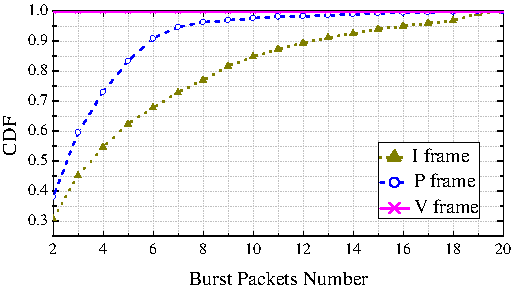
\includegraphics[width=\linewidth]{burst-frame}
	\caption{Different number of burst packets for different frames.}
	\label{fig:burst-frame}
	\termspace
\end{figure}
\fi

\subsection{Timeout retransmission of video frames}
\label{sub:timeout-frame}

If the fast retransmit can not recover a lost packet, it has to trigger timeout retransmission~\cite{flach2013reducing}. According the situation when the timeout retransmission happens, the timeout retransmission can be divided into several types. If the fast retransmit packet is drop by the network, timeout retransmission has to be triggered and we refer this timeout retransmission as double retrans. If the lost packet is the last three packets of the flow, there are not enough duplicate acknowledgments (dupacks) to trigger fast retransmit, we refer it as tail retransmission. Less dupacks to trigger fast retransmit may also because the server sends less than 4 packets out(either because there are not enough packets or the cwnd is small), and we refer it as less pkt retransmission. The ACK delay/loss or all of the packets send out lost will also result in timeout retransmission, as at both of the two situations no dupacks can be produced. We refer the two timeout retransmissions as  ACK delay/loss and continuous loss respectively. 

Table~\ref{tbl:time-out-frame} shows the time of each type of timeout retransmission for I, P and V frame. Those that cannot be classified into any of the above type of timeout retransmission is refered to as others. For all of the frames, the double retrans contributes the largest part of the timeout retransmission, 46.8\% for I frame, 44.7\% for P frame and 47.2\% for V frame. That is because when the network drops a packet, the network has high probability to become congested so the fast retransmit packet also has high probability to be dropped. For V frame, less pkt retransmission is 30.8\%, much higher than I and P frame which is 11.4\% and 20.2\% respectively. As the V frame is less than one MSS, when sending the V frame, there are often few packets in the network compared with sending I frame. That not only explains why less pkt retransmission is much higher for V frame, but also shed light on voice frame's high timeout retransmission rate in Table~\ref{tbl:frame-info}. In Table~\ref{tbl:frame-info} the V frame has smaller packet loss rate but higher timeout retransmission rate. The I and P frame has high burst packet number, the time that it is stored in the router is longer that V frame, so for I and P frames the ACK delay/loss timeout retransmission are 19.1\% and 15.1\%, much higher than V frame. Also because the different burst packet number, the continuous loss for V frame is 0, while 4.2\% and 1.5\% for I and P frame respectively.


\begin{table}[ht]
\tablefontsize
\renewcommand{\arraystretch}{\assize}
 \setlength{\tabcolsep}{3pt}
\caption{Timeout retransmission analysis for different frames.}
\centering
\begin{tabular}{c|c|c|c}
	\toprule
	 timeout retrans. type & I frame(\%) & P frame(\%) & V frame(\%)\\
	\hline
	tail retrans. & 3.8 & 4.0 & 5.0 \\
	\hline
	less pkt retrans. & 11.4 & 20.2 & 30.8 \\
	\hline
	double retrans. & 46.8 & 44.7 & 47.2 \\
	\hline
	ACK delay/loss & 19.1 & 15.1 & 8.5 \\
	\hline
	continuous loss & 4.2 & 1.5 & 0 \\
	\hline
	others & 14.7 & 14.4 & 8.5 \\
	\bottomrule
\end{tabular}
\label{tbl:time-out-frame}
\termspace
\end{table}  


